\title{Final for Algebra-Based Physics: Electricity and Magnetism (PHYS135B)}
\author{Dr. Jordan Hanson - Whittier College Dept. of Physics and Astronomy}
\date{\today}
\documentclass[10pt]{article}
\usepackage[a4paper, total={18cm, 27cm}]{geometry}
\usepackage{outlines}
\usepackage{graphicx}
\usepackage{amsmath}
\begin{document}
\maketitle

\section{Equations and constants}

\begin{enumerate}
\item Volume of a sphere: $V_s = \frac{4}{3}\pi r^3$.
\item Density, mass and volume: $m = \rho V$.
\item Charge density, charge and volume: $Q = \rho V$.
\item Coulomb force: $\vec{F}_C = k \frac{q_1 q_2}{r^2}\hat{r}$.
\item Centripetal force: $\vec{F} = \frac{mv^2}{r}$
\item Definition of electric field: $\vec{F}_C = q\vec{E}$.
\item Voltage and electric field, one dimension, uniform field: $|E| = - \frac{\Delta V}{\Delta x}$.
\item Charge and capacitance: $Q = CV$.
\item Definition of current: $I = \Delta Q / \Delta t$.
\item Parallel plate capacitor: $C = \frac{\epsilon_0 A}{d}$.
\item Ohm's Law: $V = IR$.
\item Adding resistors \textit{in series}: $R_{tot} = R_1 + R_2$ \textit{in parallel}: $R_{tot}^{-1} = R_1^{-1} + R_2^{-1}$.
\item Adding capacitors \textit{in parallel}: $C_{tot} = C_1 + C_2$ \textit{in series}: $C_{tot}^{-1} = C_1^{-1} + C_2^{-1}$.
\item Electrical power: $P = IV = I^2 R = V^2/R$.
\item Magnetic dipole moment: $\vec{\mu} = I \vec{A}$, where $\vec{A}$ is the area vector. $\mu = N I A$ if there are $N$ loops.
\item Torque on a magnetic dipole: $\tau = \vec{\mu} \times \vec{B}$.  The magnitude is $\tau = \mu B \sin(\theta)$.
\item Hall voltage: $emf = B l v$.
\item Definition of magnetic flux: $\phi_m = \vec{B} \cdot \vec{A}$.  The units are T m$^2$, which is called a Weber, or Wb.
\item Faraday's Law: $emf = -N \frac{\Delta \phi}{\Delta t}$.
\item Faraday's Law using \textbf{Inductance}, M: $emf = -M \frac{\Delta I}{\Delta t}$.
\item Typically, we refer to \textit{mutual inductance} between two objects as $M$, and \textit{self inductance} as $L$.
\item Magnetic permeability: $\mu_0 = 4\pi \times 10^{-7}$ T m A$^{-1}$
\item Units of inductance: V s A$^{-1}$, which is called a Henry, or H.
\item Coulomb constant: $k = 8.9876 \times 10^{9}$ N m$^2$ C$^{-2}$.
\item Fundamental charge: $q_e = 1.602 \times 10^{-19}$ C.
\item Speed of light: $\approx 3 \times 10^{8}$ m/s.
\item Permittivity of free space: $\epsilon_0 = 8.85 \times 10^{-12}$ N$^{-1}$ C$^2$ m$^{-2}$.
\end{enumerate}

\clearpage

\section{Exercises}

\begin{enumerate}
\item \textbf{Chapter 18: Electrostatics}
\begin{enumerate}
\item 
\begin{figure}
\centering
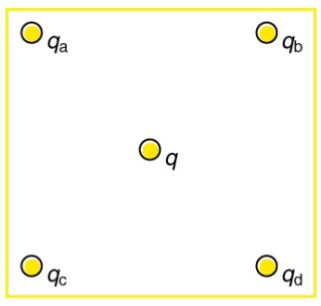
\includegraphics[width=0.25\textwidth]{charges.png}
\caption{\label{fig:charges} Five charges arranged in a square with one in the middle.}
\end{figure}
Five charges are arranged as in Fig. \ref{fig:charges}, and the side length is 1 cm. (a) If $q_a = q_b = q_c = q_d$, what is the net force on the central charge, $q$? (b) If $q_a = q_b = 1$ nC, and $q_c = q_d = -1$ nC, what is the \textit{electric field} at the center where $q$ is located?  (c) If $q=2$ nC, what is the magnitude and direction of the force on $q$? \\ \vspace{4cm}
\item Draw the electric field of the charge distribution in Fig. \ref{fig:charges} if (a) all charges have +1 nC, and (b) if $q_b$ and $q_c$ have -1 nC but the other three have +1 nC.  (c) Assuming $q_b$ and $q_c$ have -1 nC but the other three have +1 nC, would the system spin clockwise or counterclockwise if an external electric field were pointed to the right? \\ \vspace{5cm}
\end{enumerate}
\item \textbf{Chapter 19: Voltage and Capacitance}
\begin{enumerate}
\item  How far apart are two conducting plates that have (a) an electric field strength of $5$ kV/m between them, if their potential difference is 15.0 V? (\textit{Pay attention to the units}). (b) Assuming the distance $d$ between the plates found in part (a), and a plate area of $A = 1$ cm$^2$, what is the capacitance? (c) For 15.0 V, how much charge is stored in this capacitor? \\ \vspace{4cm}
\item
\begin{figure}
\centering
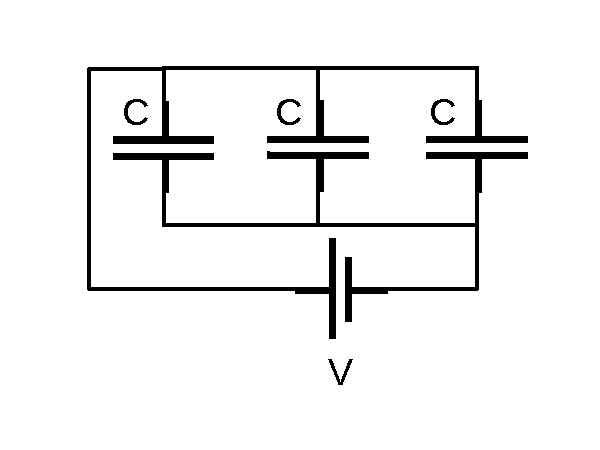
\includegraphics[width=0.3\textwidth,trim=0cm 1cm 0cm 0cm,clip=true]{iV3.pdf}
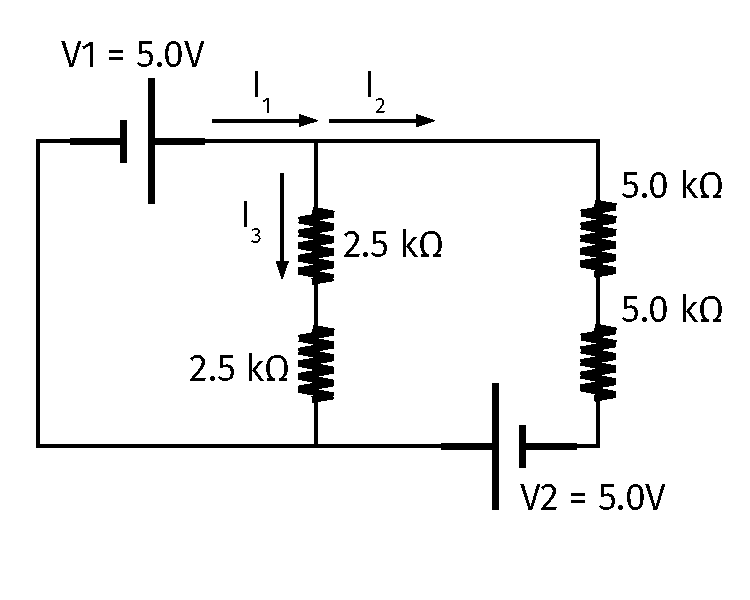
\includegraphics[width=0.3\textwidth]{iV4.pdf}
\caption{\label{fig:circuit} (Left) Three capacitors and a battery in a circuit. (Right) A circuit with two batteries and four resistors.}
\end{figure}
If $C = 1\mu$F and $V = 12.0$ Volts in Fig. \ref{fig:circuit} (left), what is the total capacitance, and (b) how much total charge is stored? \\ \vspace{1.5cm}
\end{enumerate}
\item \textbf{Chapters 20-21: Current, Resistance, and DC Circuits}
\begin{enumerate}
\item A couple are renovating a room in their house.  They replace three incandescent 50W light bulbs with two 10W LED bulbs that cost \$15.00 each.  In their area, energy prices are \$ 0.16 per kilowatt-hour.  (a) Calculate the cost to run the three 50W bulbs for 720 hours (\textit{Pay attention to units}).  (b) Calculate the cost to run the two 10W LED bulbs for 720 hours.  (c) What is the difference in cost? (d) \textbf{Bonus point:} How many hours would it take to have a difference of \$30.00, which woud recoup the cost to switch to LEDs? \\ \vspace{2cm}
\item Solve for the (a) currents in Fig. \ref{fig:circuit} (right). (b) Using $\Delta Q = I \Delta t$, how much charge is drained from battery $V1$ in 12 hours? (c) How much charge must $V1$ have if we want it to run for 24 hours? \\ \vspace{6cm} 
\end{enumerate}
\item \textbf{Chapter 22: Magnetism}
\begin{enumerate}
\item A Hall effect flow probe is placed on an artery, applying a 0.2 T magnetic field across it. What is the expected Hall voltage, given that the blood vessel's diameter is 4.0 mm and the blood velocity is 5 mm/s? \\ \vspace{1cm}
\item An AC motor is built with $N=500$ coils each having an area of 20 cm$^2$.  The coils are rotating inside a magnet of 0.2 T.  What is the maximum torque achieved by this motor? \\ \vspace{2cm}
\item
\begin{figure}
\centering
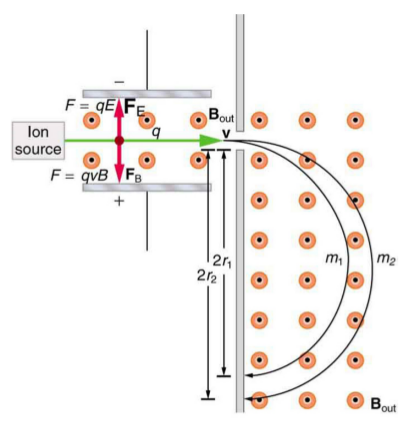
\includegraphics[width=0.3\textwidth]{select.png}
\caption{\label{fig:selector} The basic schematic of a \textit{velocity selector}, in which charged particles move through perpendicular E and B-fields. Only particles with $v = E/B$ travel through to the right portion.  Once there, centripetal force is provided by the Loretnz force, and particles of different mass curve with different radii.}
\end{figure}
In Fig. \ref{fig:selector} a velocity selector is depicted.  If $E = 10^4$ V/m and $B = 10^{-2}$ T, (a) what is the velocity of the particles that travel through to the right portion of the device? (b) If a particle traveled at the speed found in part (a) in a B-field that was 1.0 T, what would be the radius of its path? \textit{Hint: set the centripetal force equal to the Lorentz force.} \\ \vspace{4cm}
\end{enumerate}
\item \textbf{Chapter 23: Electromagnetic Induction and Inductance}
\begin{enumerate}
\item Suppose we need an inductor that produces an emf of 5.0 V for a current that changes at a rate of 125 A/s.  What inductance do we need? \\ \vspace{1cm}
\item A large research solenoid has a self-inductance of 25.0 H. What induced emf opposes shutting it off when 100 A of current through it is switched off in 80.0 ms?
\end{enumerate}
\end{enumerate}

\end{document}